% The corner transfer matrix environment of one site of an infinite
% two-dimensional network.
%
% Everything outside the site is contracted into eight tensors: four corners
% C, each a quarter of the plane, and four sides T, each a half-row or
% half-column running off to infinity. They are the environment, and drawn in
% its colour. CTMRG grows them by absorbing a row or column of the lattice into
% the sides and corners and truncating with projectors, until they stop
% changing; then a local expectation value is this picture with the operator
% put into the middle.
%
% a is the site in the middle: for a PEPS, the tensor and its conjugate joined
% along the physical index, so its bonds are double -- and the bonds between C
% and T are the environment's own, of dimension chi.
\documentclass[border=4pt]{standalone}
\usepackage{amsmath,amssymb}
\usepackage{tikz-tensors}
\input{notation}
\begin{document}
\begin{tikzpicture}
  \tnstack{E}{3}{top, mid, bot}
  \tnlayer{E}{top}{corner/$C$, side/$T$, corner/$C$}
  \tnlayer{E}{mid}{side/$T$, coef/$a$, side/$T$}
  \tnlayer{E}{bot}{corner/$C$, side/$T$, corner/$C$}
  \tnconnect{E}
  \tnmid{E-top-1}{E-top-2}{$\chi$}
\end{tikzpicture}
\end{document}
